% \addtocontents{toc}{\vspace{31\baselineskip}} % This line moved the Chapter 5 TOC entry to the next page to be with it's subheadings.

\chapter{Tool Wear Classification for Conical Picks
using Acoustic Fourier Spectra Magnitude \label{chap:P2}}

\begin{center}
    Modified from a paper to be published in The Journal of ABC\footnote{Reprinted with permission of J. of ABC, 25(1), 41-45.}.
    
    Jane Jones\footnote{Graduate student and Associate Professor, respectively, at the Colorado School of Mines \label{note1}}$^,$\footnote{Primary researcher and author}, Sam Smith\footnote{Different Institution and position}, Ann Adams$^{\ref{note1},} $\footnote{Author for correspondence}
\end{center}

\subsection{Abstract}

Underground coal mine workers who operate continuous mining machines 
rely on many cues to determine tool wear. 
This skill is difficult to train and proximity to the
mining interface is a hazard to the machine operators. 
To create safer conditions for machine operators, we propose an acoustic classification method for determining tool wear.
To demonstrate this technique, we cut a concrete sample with conical picks of different wear levels
 using a linear cutting machine and record the acoustic data for classification experiments.
We highlight the differences in acoustic frequency spectra and
 demonstrate classification of short segments of the recorded acoustic data, less than 100 milliseconds in duration,
using three popular classification techniques: the K-nearest neighbors classifier, 
 the support-vector machine classifier, and the multi-layer perceptron classifier. 
We compare the performance of the techniques and also examine the effects of segment size and downsampling.
Of our tested methods, the support-vector machine gives good performance with little complexity.
This technology could aid operators in performing their roles from a safer distance, 
alerting them to worn tool conditions in real time.


\subsection{Introduction}\label{sec1}

Underground mining safety has not improved over the last decade, with the rate of fatalities
per 100,000 Full Time Equivalent (FTE) workers remaining around 21.4 from 2011 to 2020 \cite{nioshdata}. 
In the literature review conducted by Sari et. al., it is noted that younger, less experienced
miners are at greater risk of suffering a disabling injury \cite{Sari2004}.
On the other hand, for older and more experienced miners, 
the high levels and long duration of exposure to the hazards inevitably leads to problems
like hearing loss \cite{Erol2022}, or other diseases such as black lung, 
a serious lung disease caused by exposure to coal dust, which can be fatal \cite{Colinent2020}.

Some examples of dangers in the underground mine environment include: 
tunnel collapse, explosive gasses \cite{Juganda2022},
high temperatures \cite{cinar2020}, exposure to diesel particulate \cite{Bugarski2022},
and the crush hazards caused by machines used for the operation \cite{Swanson2019}.
Machine operators in underground coal mines are particularly at risk,
as they must remain near the cutting interface to pick up cues from machine and the environment
to monitor cutting conditions \cite{Bartels2009}.
Workplace accidents caused by these hazards is problematic and they lead to 
loss of productivity, worker injury, and loss of life \cite{sensogut2021}.
The National Institute for Occupational Safety and Health (NIOSH), 
recommends removing workers from hazardous locations as the best form
of risk reduction in general \cite{niosh_2015}.

Aiding operators with improved sensors for tool wear detection can help them 
perform their role from a greater distance to the cutting interface and 
reduce their risk from dust exposure as well as the from the immediate dangers at the cutting interface.
Experienced operators are an invaluable resource, 
 as they hold the experience gained after years of dealing with hazardous conditions \cite{Bartels2009}.
Operators are known to rely on many cues, including visual, acoustic, and vibrational.
This suggests a sensor can measure these cues.

Acoustic sensors can operate with a quick, less than one second, response time and detect changes in 
material type and tool wear in many domains \cite{Zakeri2017, Zhong2013, Rad2014, Zakeri2015}.
When comparing acoustic, visual, and vibrational cues for tool wear,
acoustic detection of tool wear has the advantage over visual detection in that it
does not require a clear line of sight to the cutting interface, 
which is often in a hazardous location near the machine \cite{Bartels2009}.
Alternatively, vibrational cues require direct contact with the cutting process, 
which requires a more robust sensor design compared to an acoustic sensor which is placed further away.
We choose to investigate using acoustic data for objective tool wear classification from a distance.

Any technology that is employed in this domain must be well suited for the task it is
designed to perform, or else its adoption is unlikely \cite{Swanson2019}.
By providing objective, real time data to human operators, 
our proposed technology can help operators make objective decisions 
regarding shutting down operations for cost-saving maintenance or continuing work.
Automating tool wear detection can also allow machine operators to focus on other aspects of machine operation, 
increasing their productivity.
Automation also enables collection of data that could be analyzed for trends in tool wear during operation.

The rest of this article is outlined as follows. 
In the Background subsection, the application background
 and previous work used to guide this study are discussed.
The Methods subsection follows, and it gives detailed description of the 
 experimental equipment, classification methods, and metrics for comparing classification performance.
After that, the Results subsection lists the notable results.
Then, a Discussion subsection is given, which states the merits of the tested methods 
 and provides recommendations for implementation.
Finally, a Conclusions subsection summarizes the work and its relevance considering the target application.

\subsection{Background}\label{sec1a}

In the black lung study by Colinent, the author notes that much effort has been given to dust mitigation.
Strategies include: minimizing dust generation, preventing dust from circulating, removing
dust from circulation, diluting dust concentration, use of barriers and ventilation direction
to reduce worker exposure, and maintenance of these systems \cite{Colinent2020}. 
The idea of removing workers from hazardous zones is supported 
 by the general advice given by NIOSH in their hierarchy of controls \cite{niosh_2015}.
In order to remove workers from the hazardous zones, they must be enabled to perform their roles from 
more remote locations. 

Considering that experienced human operators are able to detect tool wear using acoustic cues
suggests that enough relevant information can be captured within the typical human hearing range.
A study on occupational hearing loss in underground mines reported that the type of hearing loss experienced 
by underground coal miners indicates a noise frequency below 6 kHz and a noise intensity 
around 90 dBA \cite{Erol2022}. 
We aim to capture these low frequency and high intensity acoustic emissions for classification.

As early as the 1990's, methods which consider the total volume of the acoustic emissions,
the count of peaks and valleys in the signal, and the changes in signal spectra 
have been researched \cite{Tan1992,Kakade1995}.
Proper preprocessing is important. 
In underground mining, the rock cutting system can lose mass as tools are worn,
resulting in a non-stationary dynamic system.
Fast Fourier transform based preprocessing of a small window of signal
 and subsequent classification with a support-vector machine has shown 
 to be an effective method for robust classification of non-stationary dynamic systems \cite{xu2016fftsvm}.

Other preprocessing techniques for similar problems include wavelet and Empirical Mode Decomposition.
Wavelet preprocessing combined with machine learning
has been used with success in recent years 
 \cite{he2013vibration, sadegh2016classification, skariah2021health}.
Empirical Mode Decomposition has demonstrated vibration classification for tool wear
 in other domains \cite{Xu2009, Nie2011, Zhan2014}.
We choose fast Fourier spectra magnitude based preprocessing and normalization for its time-invariant properties,
small number of hyperparameters, and known effectiveness across domains \cite{Xu2016, Harlianto2022}.

Both wavelets and Empirical Mode Decomposition are time-variant.
The wavelet transform is known to be very sensitive to small time translations \cite{Yen1999}.
With wavelets, this can be mitigated by measuring the average energy for 
a continuum of offsets and using those values 
as the feature vector for classification \cite{Baccar2015}.
Similar processing would be needed for Empirical Mode Decomposition. 
Another option is to register the signal in the time domain to an event, such as contact with the material.

We motivate our choice of preprocessing methods with the idea that different tool wear levels in a conical pick
will produce different acoustic emissions with different Fourier frequency spectra magnitude for a given material. 
We verify this by analyzing objective differences in statistical distributions 
of the frequency spectra magnitudes for the tested categories.
To leverage these differences, we employ and compare different classification techniques.
These methods and how they are compared are described in the next subsection.

\subsection{Materials and Methods}\label{sec2}

A homogeneous concrete sample is cut using the Linear Cutting Machine
at the Earth Mechanics Institute at the Colorado School of Mines, shown in \ref{fig:setup},
and capable of testing with many cutting tools \cite{THYAGARAJAN2024105675}. 
Acoustic data is recorded at a sample rate of 44.1 kHz using a digital camcorder,
and then the data is categorized by tool wear condition.
The different tool wear levels are shown in \ref{fig:levels}.
The tool tips have been artificially worn with a lathe to a spherical shape to approximate even wear.
They vary in diameter and have been chosen to represent a new, a moderately used, and a worn tool.

\begin{figure}[t!]
\centering
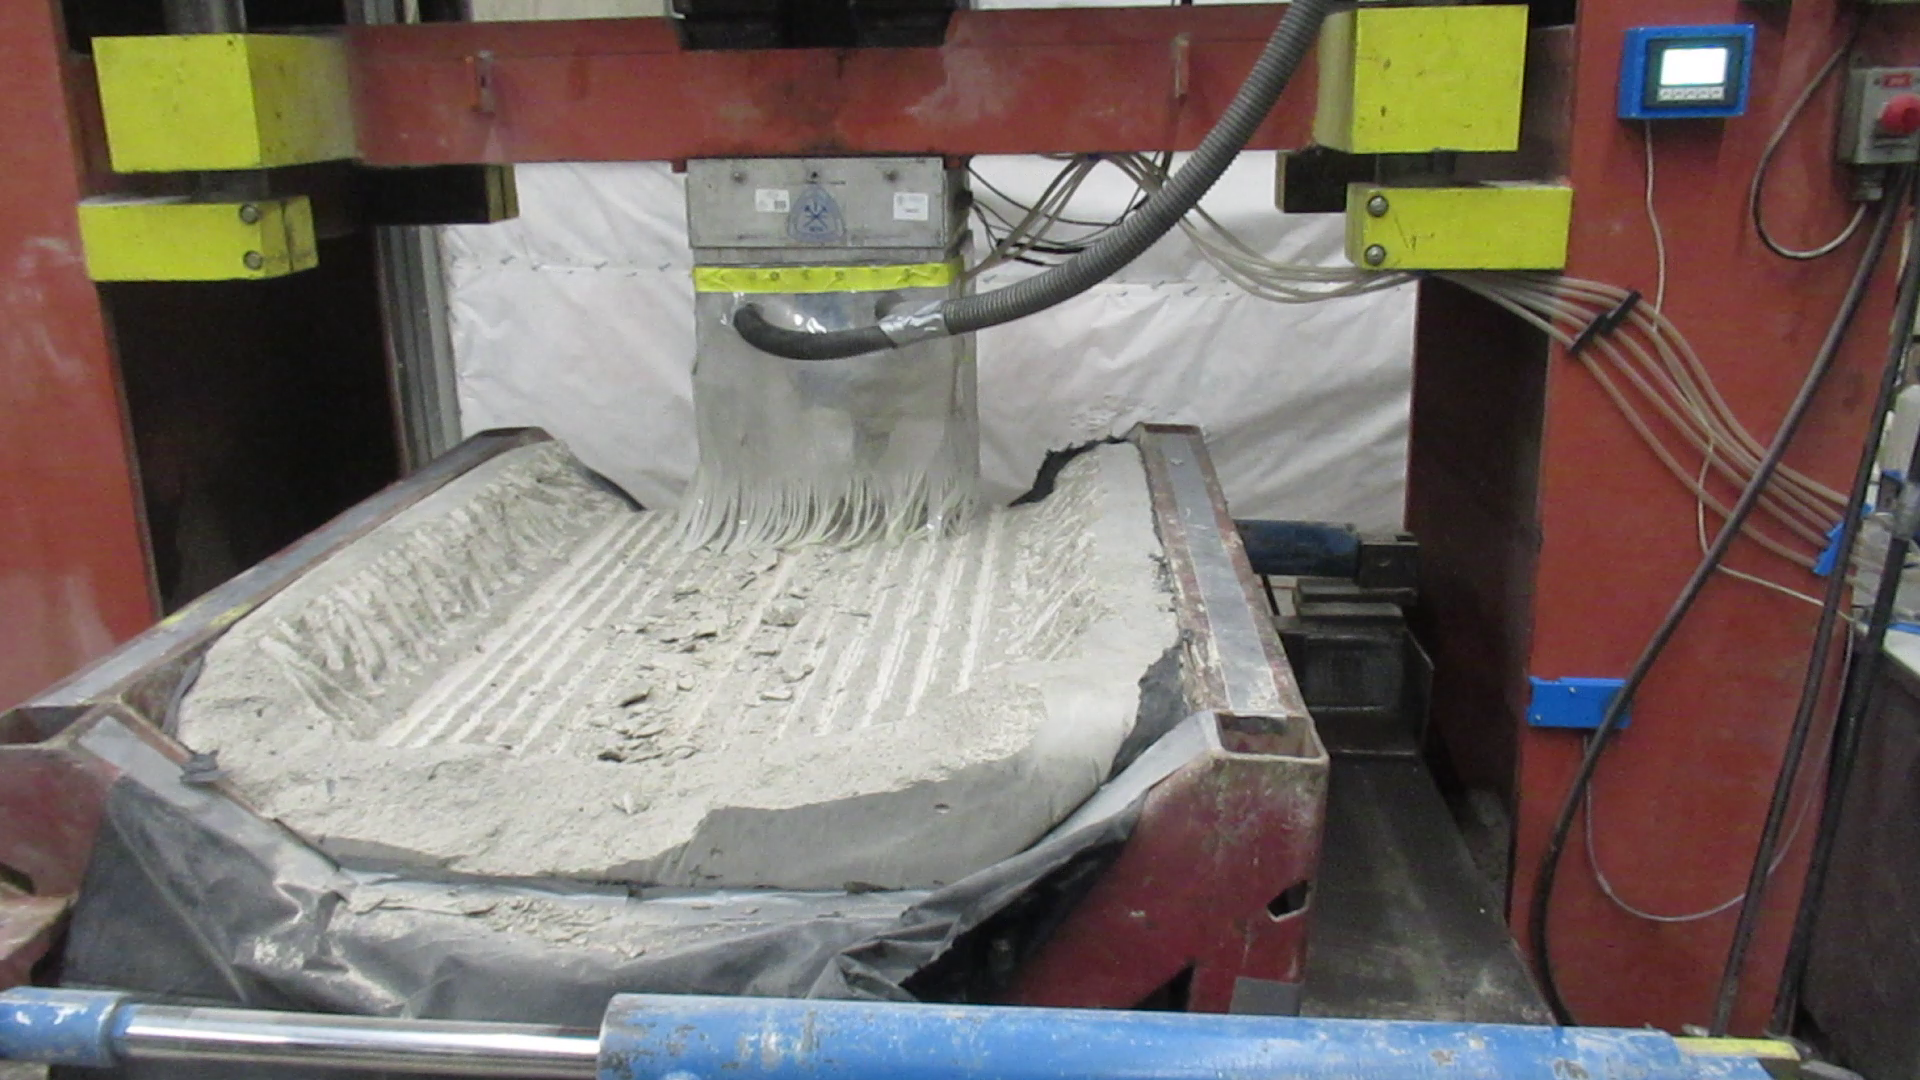
\includegraphics[width=5.5in]{p2_media/figures/raw/setup.png}
\caption{The Linear Cutting Machine at the Earth Mechanics Institute of Colorado School of Mines.
Hydraulic actuators move the rock box for positioning and cutting. The rock sample in this experiment
is a solid block of concrete. This is a homogeneous material that will isolate the changes in tool wear.
Additional equipment consisting of a dust shroud and vacuum sample collection system was used for a
 simultaneous study on dust generation, but not for this study.
Forces are recorded using integrated load cells in the coupling between the tool and the frame.
The acoustic signals for this experiment were recorded from the camcorder used to take this image.
}
\label{fig:setup}
\end{figure}

\begin{figure}[t!]
\centering
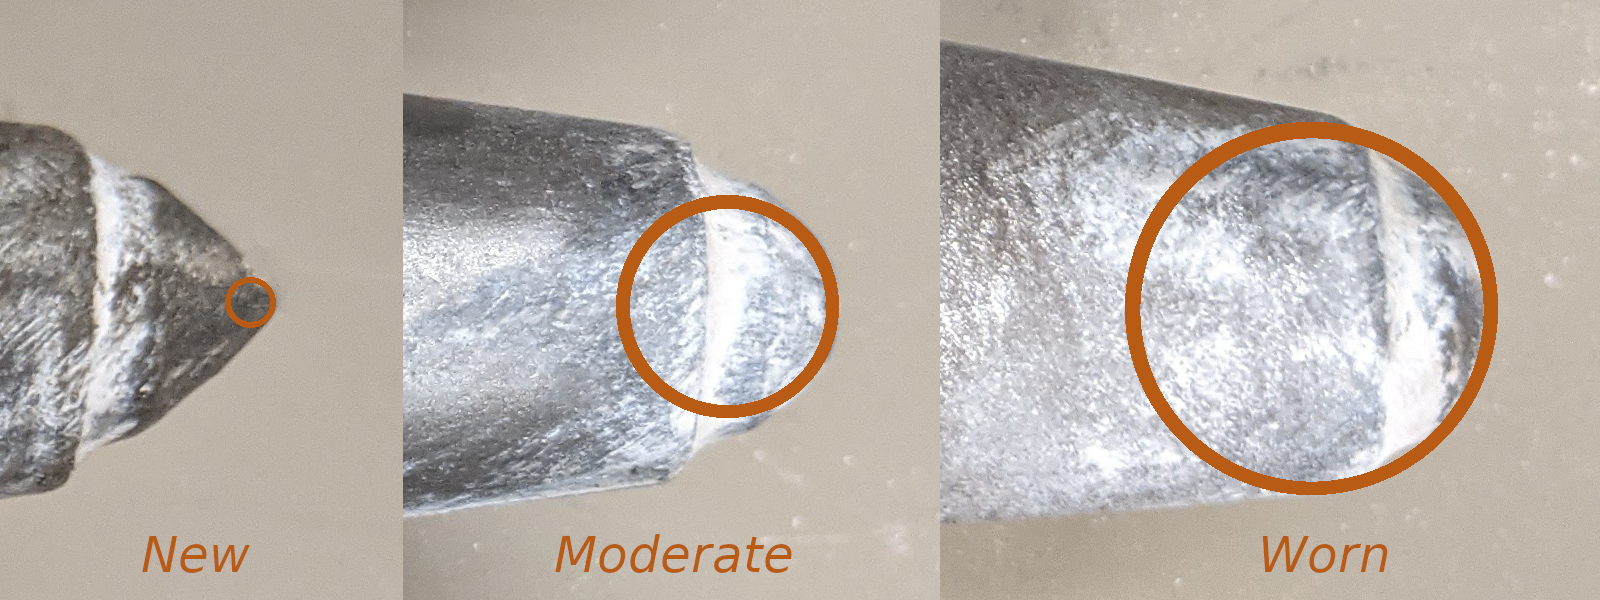
\includegraphics[width=5.5in]{p2_media/figures/tips.png}
\caption{The tips of the conical picks with different wear levels used for the experiment.
The tips are worn to a spherical shape to approximate even wear. The \textit{new} tool is unmodified
and has a diameter of 3.71mm, the \textit{moderately} worn tool has a diameter of 17.9mm,
 and the \textit{worn} tool has a diameter of 27.5mm. The tool tips were artificially worn down using a lathe.}
\label{fig:levels}
\end{figure}

The sample is cut by layers, with each layer consisting of several lines spaced roughly three centimeters apart.
The cutting speed is set to 10 inches per second and penetrations of 1.5 and 2.0 inches are used.
For each wear category, we collected four lines for both penetrations. 
To reduce edge effects of our experiment, 
like the differences in impulse response
between the linear cutting machine and our sensor,
we trim the recording of each line to 6 seconds,
starting shortly after the bit hits the material. 
We chop the data into small segments of 20, 40, 60, 80, 100, and 200 milliseconds in duration.
The segments are allowed to overlap by 50\%, and
this yields roughly 480 samples for the 100 millisecond case and 
4800 samples for the 20 millisecond case for each wear category.

The fast sampling rate of our microphone, 44.1 kHz, means that even short segments,
dozens of milliseconds in duration, will have thousands of data points.
Reducing input dimension via downsampling after low pass filtering will preserve 
low frequency data while leading to faster processing for the classification algorithms and 
eliminate additional aliasing.
These segments also have a Hamming window applied to enforce periodic assumptions of the Fourier based preprocessing.
Longer signal windows will yield more resolution in the frequency domain up to the sampling frequency
while higher sampling rates offer slightly increased resolution but over a wider frequency range.
Our study compares the effect on classification performance from both downsampling and window length.

We score the methods using the F1 score, which penalizes false positives and false negatives,
by generating a distribution of scores and comparing the distributions \cite{Goutte2005}.
We also examine the confusion matrices of the classifiers to understand 
how the classifier is performing \cite{Bramer2007}.
Each window size data set is divided randomly in a 70:30 test train split 40 times 
to collect statistical distributions of the scores for each classification method 
when using a small sample for training data.
The preprocessing and classification methods are described in more detail below.

\subsubsection{Preprocessing}

After filtering, downsampling, and splitting the data into small segments,
the input to each of the classification algorithms is a vector of floating point numbers 
which represents a small segment of the audio recording from the cutting experiment. 
We denote a segment of the data, starting at time $t$, as $\ora{x_t}$.
This vector has consecutive samples of the time domain signal starting at time $t$ and 
ending at the end of the window duration offset by the start time.
The first preprocessing step is to multiply this vector element-wise with a Hamming window, $\ora{h}$, and
the new vector is given as: $\ora{y_t} = \ora{h} \circ \ora{x_t}$.
The exact choice of window function has subtle effects on the algorithm performance, 
but in general the window function serves to enforce the periodic signal assumption of the 
discrete Fourier transform \cite{Harris1978}. 

After the window is applied, the Fourier based preprocessing begins.
The datasets are split 70:30 into the test and train sets. 
We denote the normalized data as $\ora{z_t}$, and it is calculated as:
\begin{align}
\ora{z_t} = (\ora{y_t} - \ora{u}) / \ora{s},
\end{align}
where both subtraction and division are performed element-wise, $\ora{u}$ represents the vector
of mean values for each dimension in the training set, 
and $\ora{s}$ represents the vector of standard deviations for each
dimension in the training set. 
The distributions of frequency spectra magnitudes and time domain waveforms
for each wear category are shown in \ref{fig:natural}.
During each experiment, the test data is normalized according to the distribution of the training set.

\begin{figure}[t!]
\centering
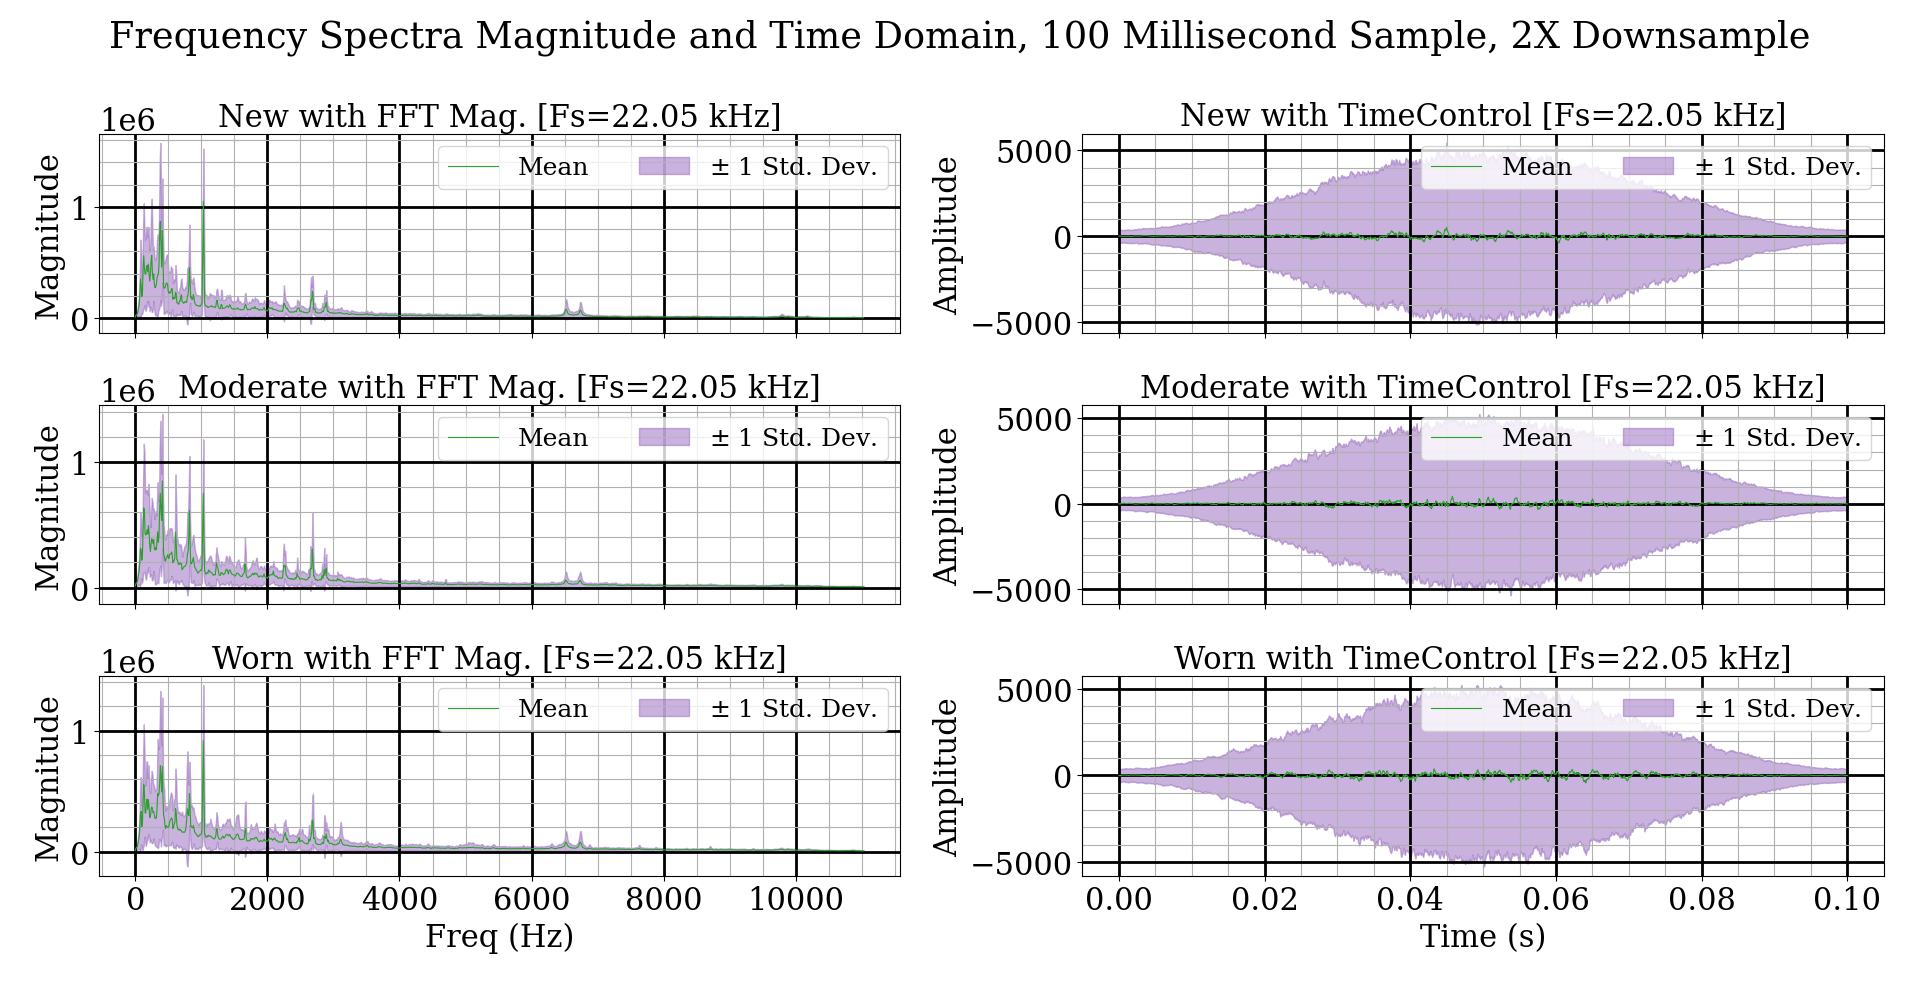
\includegraphics[width=5.5in]{p2_media/figures/raw/fig3_5_natural.png}
\caption{
The natural distribution of frequency spectra magnitude 
and time domain data of each wear category for our collected data.
The Fourier transform data has most of its energy below 4 kHz.
The higher frequency data has smaller variance compared to the
lower frequency data.
The time domain data is roughly shaped like the window function.
Transforming the time domain data into the frequency domain highlights
the changing modes between the categories.
These differences in resonant frequencies are made more apparent after normalization.
}
\label{fig:natural}
\end{figure}

Before invoking any classifiers, we can show here that there are 
objective differences in acoustic spectra across wear categories 
by performing a classic two-sided Welch-Satterthwaite t-test on each frequency bin \cite{Tamhane2000}.
The results of this test and the normalized frequency spectra magnitude distributions
for each wear category are shown in \ref{fig:sigs}.
The classification techniques discussed in the next subsection use these differences to 
determine the wear category of a given sample based on the training data.

\begin{figure}[t!]
\centering
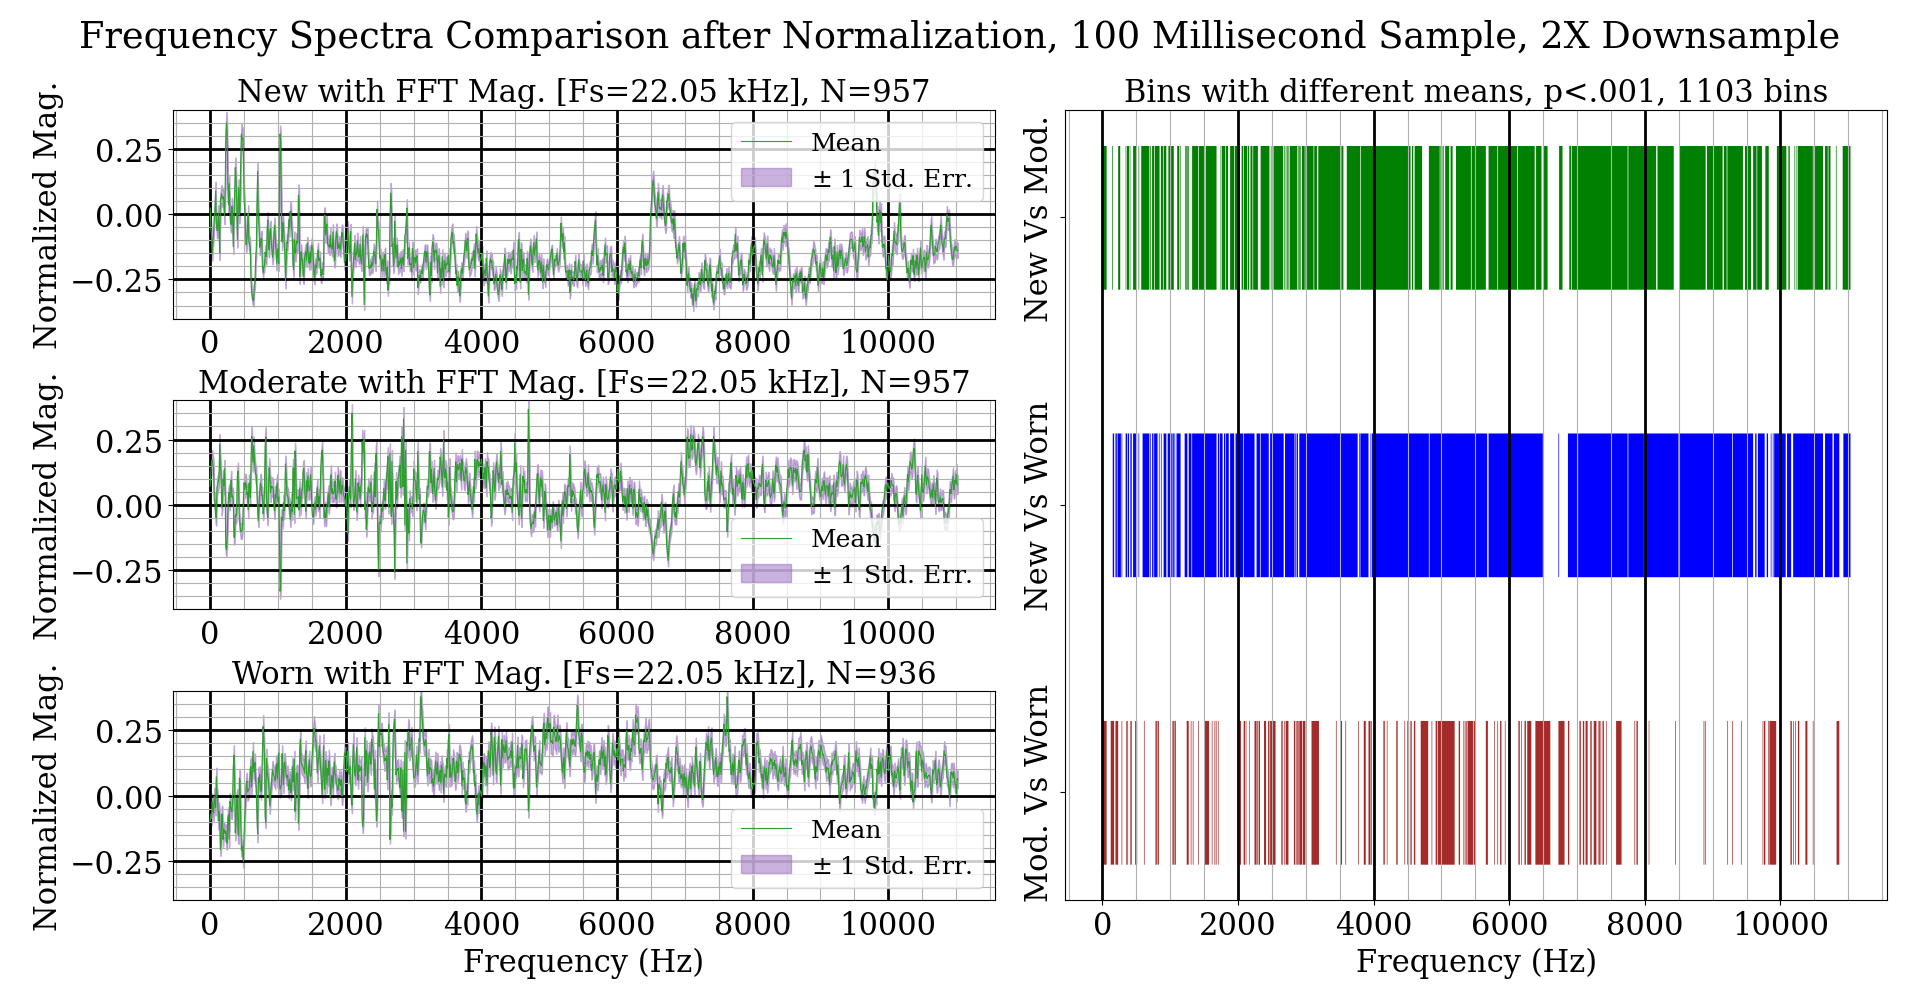
\includegraphics[width=5.5in]{p2_media/figures/raw/fig4_normalized.png}
\caption{
The mean frequency spectra magnitude after normalization for each wear category and a 
comparison between the categories for significant differences.
In the left column, the mean value and the standard error of the mean are shown for our collected data.
In the right column, the results of a t-test for each bin for each pair of categories is shown.
It is known that operators use acoustic signals to determine cutting conditions,
and this figure demonstrates significant, $p < 0.001$, differences across tool wear categories
for most frequency bins. Even though the higher frequencies have less energy, their differences
are still significant due to their low variance.
The exact changes will depend on the machine and the entire set of cutting conditions, but 
for a given environment, these differences can be observed and detected.
}
\label{fig:sigs}
\end{figure}

\subsubsection{Classification}

These data splitting, preprocessing calculations, and classification techniques are 
computed using the scikit-learn, a.k.a. sklearn, library \cite{JMLR:v12:pedregosa11a}.
The library supports many classification and regression methods and facilitates rigorous comparison.
For this study, we choose to compare the support-vector machine technique with a more simple method
and a more sophisticated method to investigate classifier efficiency. 
The more simple method is the k-nearest neighbors classifier.
The k-nearest neighbor technique works by comparing the input sample to its memory of the $k$ closest training samples, 
 and the most popular class is elected as the output.
The more sophisticated method, the multi-layer perceptron classifier, works by training a 
 network of artificial neurons to develop a series of vector transformations which results
 in accurate classification. Meanwhile, the support-vector machine aims to find a separating
 hyperplane in a transformed version of the data. 

To measure the performance of our chosen algorithms, the F1 score is 
used to evaluate the classification results. 
There is an inherent trade-off between precision and recall in practical classifiers \cite{buckland94}.
The F1 score is the geometric average of
precision and recall, and serves to evaluate overall performance. 
More detailed descriptions of the individual classification algorithms follow below.

\subsubsection{K-Nearest Neighbors}

The non-parametric k-nearest neighbors approach is used in classification 
and regression \cite{Vaishnnave12019}.
The K-nearest neighbors classifier aims to predict the class label, $g_t$ of 
future data point $x_0$ on the predetermined $q$ classes given a set 
of $p$ labeled classes $\{(x_t, g_t), t \in 1 \ldots p\}$ \cite{Song2007}. 
In order to obtain the class label for $x_0$, the K-nearest neighbor (KNN)
 classification algorithm searches for the sample's K closest neighbors 
 and then assigns the class of the majority.
The selection of K and the distance measure used are the two factors 
that have the biggest impact on a KNN classifier's performance \cite{Alf2019}. 
Without prior knowledge, Euclidean distances are typically used by the KNN classifier 
as the distance measure. These distances are simple to compute and if the data
categories are distinct, than this method will work well.
We use the Euclidean distance and $K=5$ for this study, with larger values of $K$ giving similar results.

\subsubsection{Support-Vector Machine}

The fundamental goal of the support-vector machine (SVM) is to build a separation hyperplane that best divides
 data examples into two classes while maximizing the minimum distance between points
 and the separation hyperplane \cite{lazarevic2009support}. 
Support-vector machines employ the structural risk minimization \cite{sewell2008structural}
 concept and seek to achieve zero misclassification error while reducing the 
 model's complexity. 
The problem statement and solution of its dual via Karush-Kuhn-Tucker conditions \cite{gordon2012karush}
is omitted here for brevity. 
For discussion, the decision function of the two class support-vector machine is listed here:
\begin{align}
h(x) = \mathrm{sign} \bigg( \sum_{s=1}^p \beta_s g_s k(x_s, x) + r \bigg),
\end{align}
where sign returns 1 if the input is greater than zero, $p$ is the number of support-vectors, 
$\beta_s$ and $g_s$ are weights, and $k(x_s, x)$ is the kernel mapping of the support-vector $x_s$ and the input, $x$, and $r$ is a bias term.
The kernel function is able to compare the input to the chosen support vectors in a space that highlights their differences.

The SVM is a binary classifier by nature, however many of the problems 
we are interested in tackling are multi-class (q-class) \cite{Oskoei08}.
 Hence a multi-class SVM approach must be adopted in that regard. 
In this study, a “one-against-one” approach \cite{Debnath2004} was employed. 
This approach trains q(q-1) binary classifiers to distinguish between two classes. 
The final output is the class that receives the most votes from 
the binary classifiers. 
The coefficients calculated during training are considered optimal for the given data. 
The SVM requires a roughly similar number of computations as the KNN, but takes extra steps to 
make the data more separable through the kernel function.
We use the Radial-Basis function for our kernel, as it is able to make nonlinear separations.

\subsubsection{Multi-layer Perceptron Classifier}
A specific type of feed-forward artificial neural network is the multi-layer perceptron (MLP)
and it is well-known for its stability, usability, and a relatively modest structure 
in tackling some tasks when compared to other structures \cite{yulita2018multi}. 
An MLP classifier analyzes the relationship between input and output 
in a set of p labeled classes. An input layer, a number of hidden layers, and an output layer 
make up the network topology of MLP \cite{molina2021classification}. 
Processing nodes known as neurons make up each layer, 
with each neuron connected to all neurons in the previous layer. 

Each neuron receives weighted inputs with a bias value, which are then 
transformed and processed by a nonlinear activation function \cite{montesinos2022fundamentals}. 
The hidden layer's output is shown in the following:
\begin{align}
s_r = t \bigg( \sum_{q=1}^p \omega_{qr} x_q + c_r \bigg), \quad \forall r \in \{1, \ldots, k\},
\label{eq:layer}
\end{align}
where the activation function is represented by $t(\cdot)$; 
the bias of the $r$th hidden units is represented by $c_r$; 
the inputs and weights between the input and hidden layer are represented 
by $x_q$ and $w_{qr}$, while $s_r$ is the hidden layer's output. 
Activation functions come in a variety of forms, including logistic sigmoid, softmax, 
hyperbolic tangent, and rectified linear unit functions \cite{sharma2017activation}. 
The output layer consists of one neuron for each class, and the output is the
probability that the input belongs to that neurons respective class.

The coefficients for the network are trained in an iterative fashion by examining 
the gradient of performance with respect to each one.
This forward pass and back-propagation process is repeated until the network finds 
a solution or the necessary number of iterations have been completed \cite{maxwell2017deep}.
This type of training requires a balance of many factors to be successful; but once trained,
the network can classify samples with a roughly similar number of computations as the other
techniques depending on the network size.
We use the rectified linear unit activation function and a network of two hidden layers 
equal in size to the input dimension, with more hidden layers giving similar results.

\subsection{Results}

The mean F1 scores are plotted against the window lengths for each of the tested methods 
at each of the tested downsampling factors.
The K-nearest neighbors classifier performance is shown in \ref{fig:perf_KNN}.
The support-vector machine classifier performance is shown in \ref{fig:perf_SVM}.
The multi-layer perceptron classifier performance is shown in \ref{fig:perf_MLP}.
In the above figures, the F1 score of a method is significantly greater than another method
if the median score is above the max score of the other method.
This comparison method is slightly more conservative but more visually straightforward
than comparing each score in the collected distribution,
as recommended in \cite{Goutte2005}.
Classifier performance was greater with longer window lengths and 
increased sampling rates, or lower downsampling factors.

Looking at the confusion matrices for the different types of classifiers generally showed
that most of the confusion was between the \textit{moderate} and \textit{worn} categories of bits, suggesting that
these two categories have responses that are more similar to each other than to the \textit{new} category.
A sample confusion matrix for a SVM classifier experiment is shown in \ref{tab:conf}, 
it is representative of most of the other classifiers too. 
It shows that there is about twice at much confusion between \textit{moderate} and \textit{worn} categories as there is 
between \textit{new} and the other two wear categories.
This indicates that determining wear to a fine degree may be difficult with acoustic emissions alone.

\begin{table}[h]
\centering
\caption{Confusion Matrix for Acoustic Wear Classifier; Normalized by true class size. \newline
         Concrete sample, 100 millisecond window, 70:30 test train split, \newline
         support-vector machine with fast Fourier transform preprocessing.}
\label{tab:conf}
\begin{tabular}{|l|lll|}
\hline
Test Result \% & \multicolumn{3}{l|}{Prediction}                            \\ \hline
True Class    & \multicolumn{1}{l|}{\textit{new}} & \multicolumn{1}{l|}{\textit{mod}} & \textit{worn} \\ \hline
\textit{new}           & \multicolumn{1}{l|}{90.15 }    & \multicolumn{1}{l|}{ 4.77}    &  5.08    \\ \hline
\textit{mod.}           & \multicolumn{1}{l|}{3.85}    & \multicolumn{1}{l|}{87.26}    &   8.89    \\ \hline
\textit{worn}          & \multicolumn{1}{l|}{5.67}    & \multicolumn{1}{l|}{9.25}    &  85.07     \\ \hline
\end{tabular}
\end{table}

%array([[0.90153846, 0.04769231, 0.05076923],
%       [0.03851852, 0.87259259, 0.08888889],
%       [0.05671642, 0.09253731, 0.85074627]]), 

%\caption{Confusion Matrix for Acoustic Wear Classifier; Normalized by prediction \newline
%         Concrete Sample, 100 millisecond Window, 70:30 test and train, SVM with FFT_Mag.}
%\begin{tabular}{l|c[table-format=2.2]c[table-format=2.2]c[table-format=2.2]|}
%{Test result \%}   & \multicolumn{3}{l|}{Prediction}                 \\ \hline
%{True Class} & \multicolumn{1}{l|}{\textit{new}} & \multicolumn{1}{l|}{\textit{mod.}} & {\textit{worn}}  \\ \hline
%{\textit{new}}        & 90.15                   & 4.77                     & 5.08 \\
%{\textit{mod.}}       & 3.85                    & 87.26                    & 8.89 \\
%{\textit{worn}}       & 5.67                    & 9.25                     & 85.07
%\end{tabular}
%\end{table}

\begin{figure}[t!]
\centering
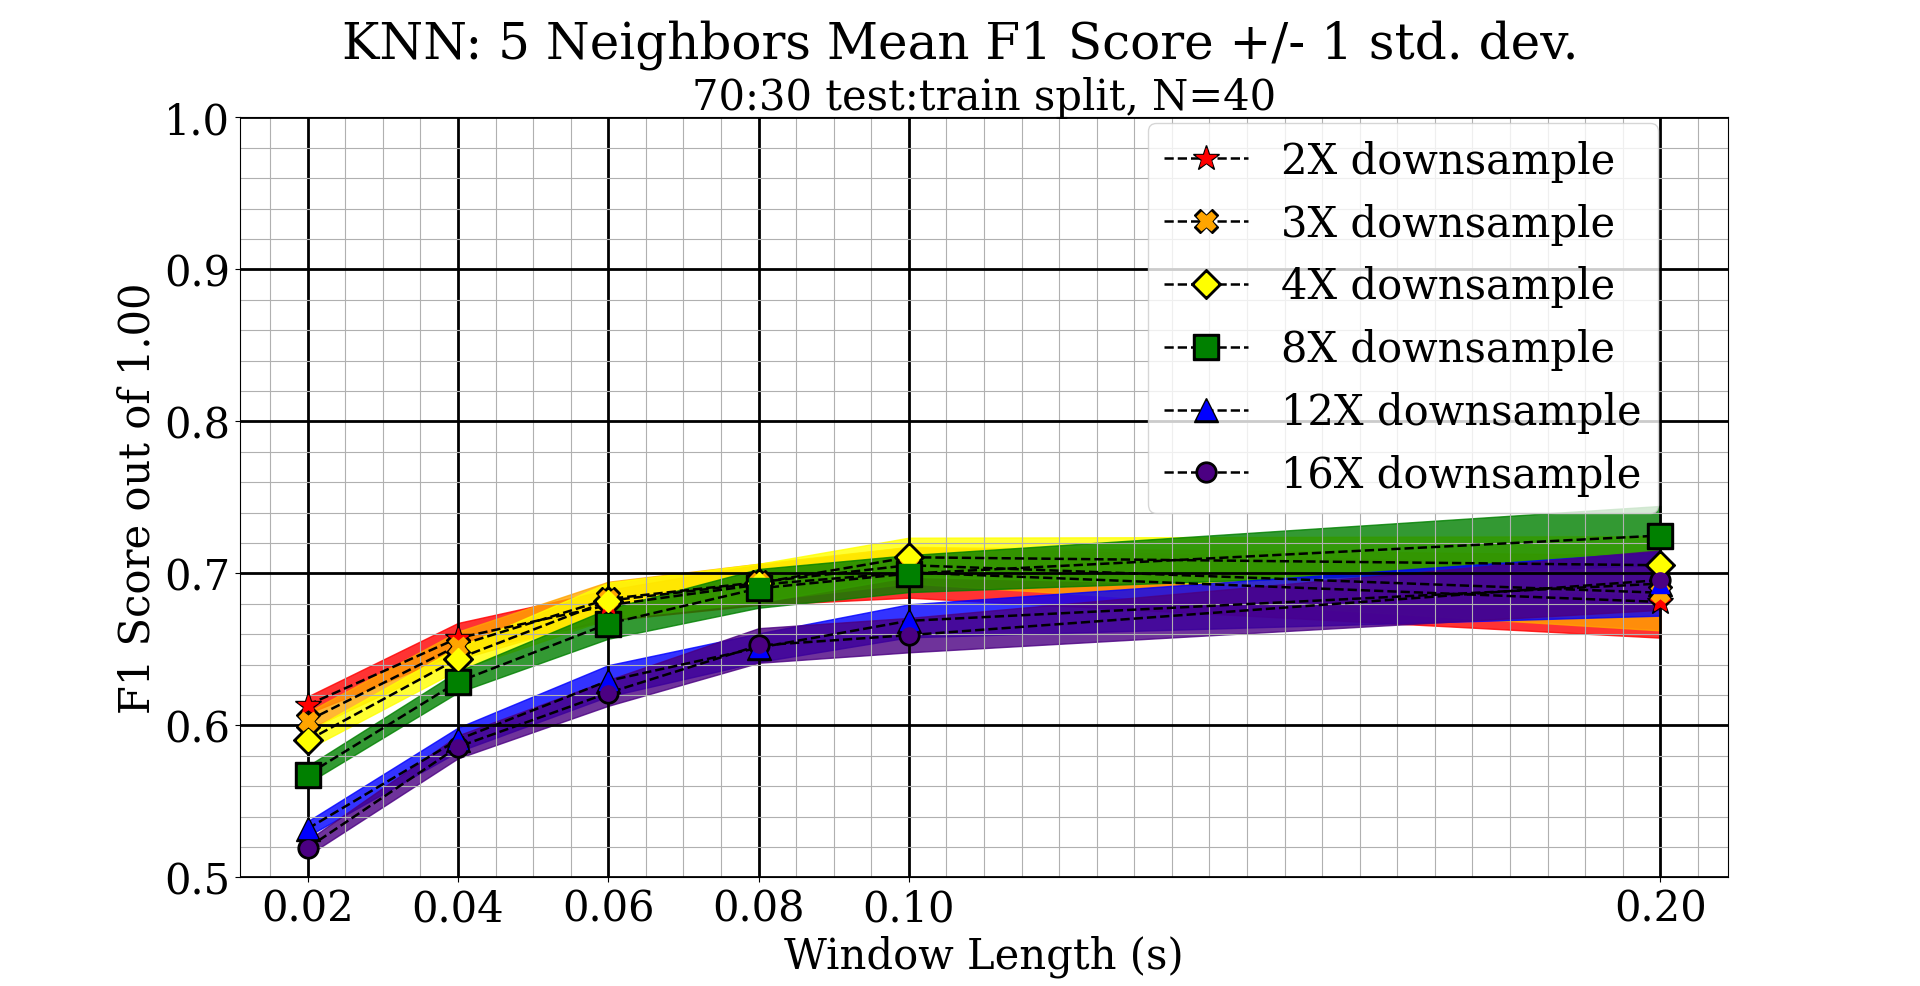
\includegraphics[width=5.5in]{p2_media/figures/raw/KNN_F1_scores.png}
\caption{The mean F1 score and standard deviation for K-nearest neighbors method. 
Using K=5 gave slightly better performance than other values, 
but this method performed the worst overall.
Increasing window length gave better performance for this method, and downsampling had little effect
for larger window lengths. 
The F1 score only increased a small amount when using the 0.2 second window compared to the 0.1 second window.
}
\label{fig:perf_KNN}
\end{figure}

\begin{figure}[t!]
\centering
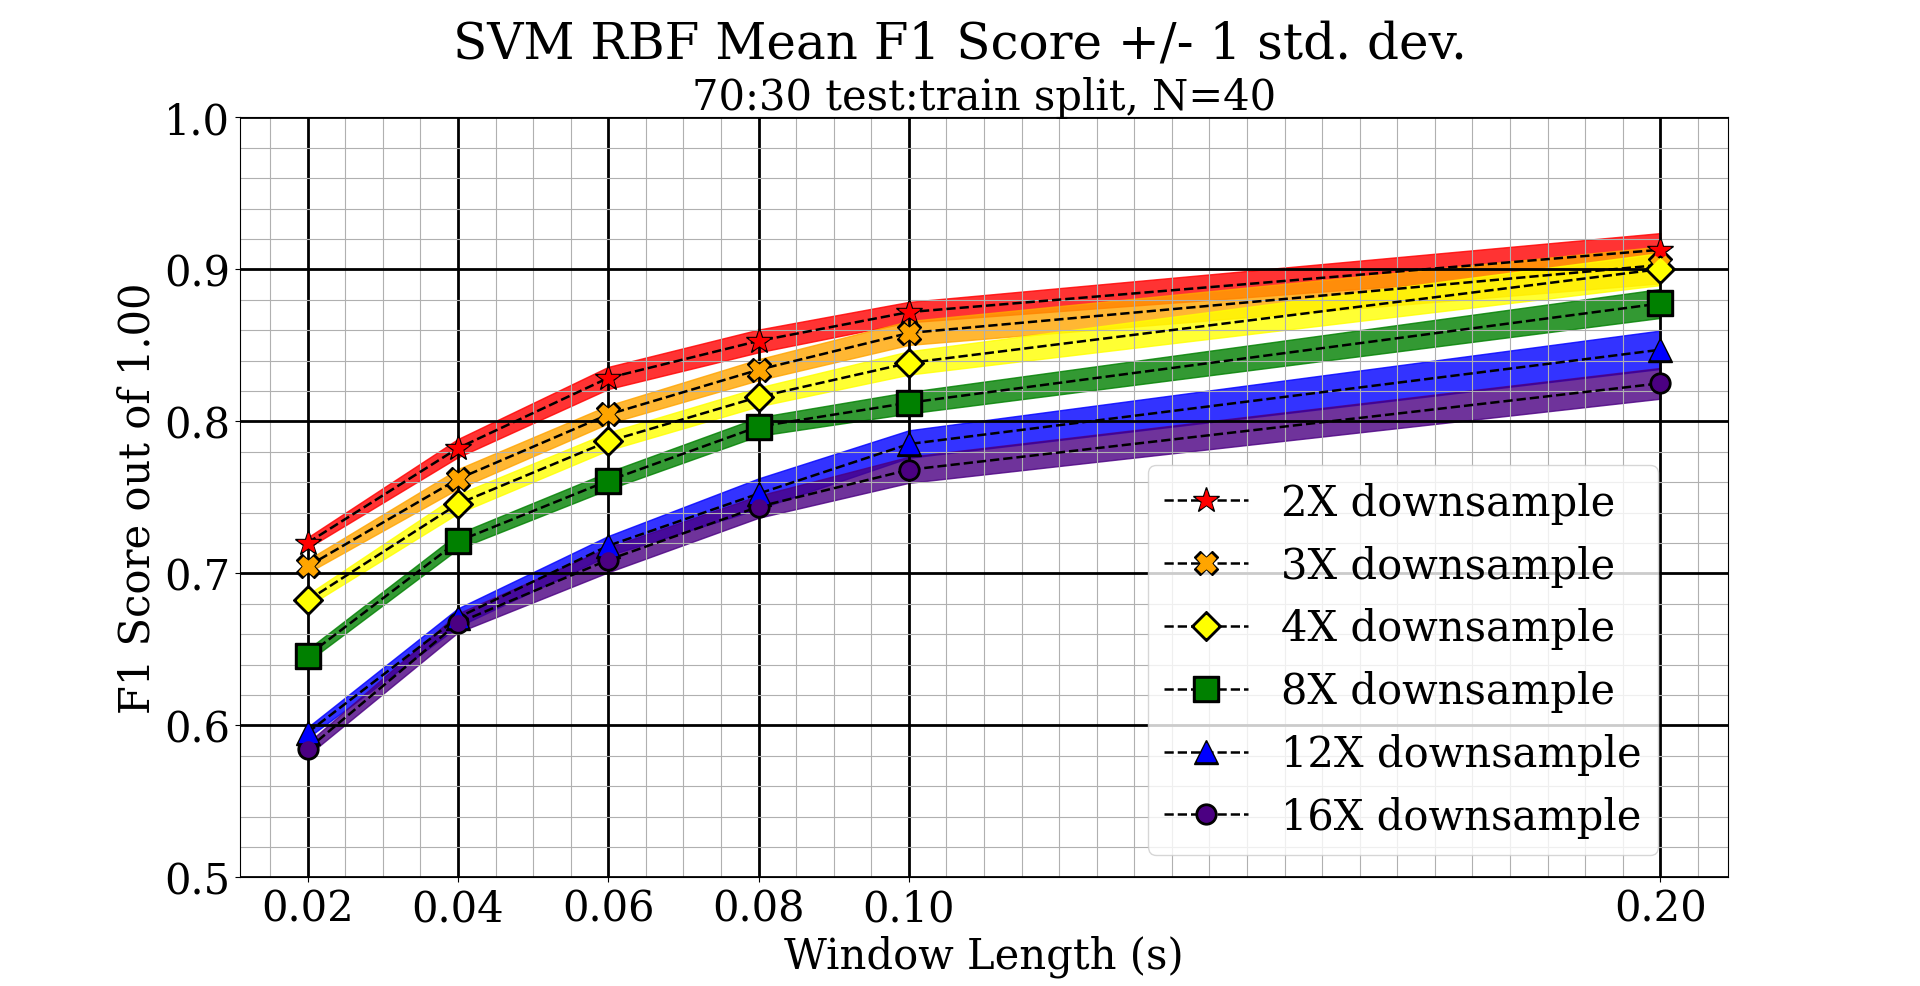
\includegraphics[width=5.5in]{p2_media/figures/raw/SVM_F1_scores.png}
\caption{The mean F1 score and standard deviation for the tested support-vector machine method.
This is a low hyperparameter method that performs very well and does so efficiently.
With this method, performance trends better with longer window length 
and higher sampling rates, or less downsampling, for our experiment.
Increasing window length gave better performance for the number of variables introduced
compared to increasing sampling rates.
Using a window length of 0.2 seconds gave the best performance of for all downsampling levels,
and the performance was similar for samples with less downsampling.
}
\label{fig:perf_SVM}
\end{figure}

\begin{figure}[t!]
\centering
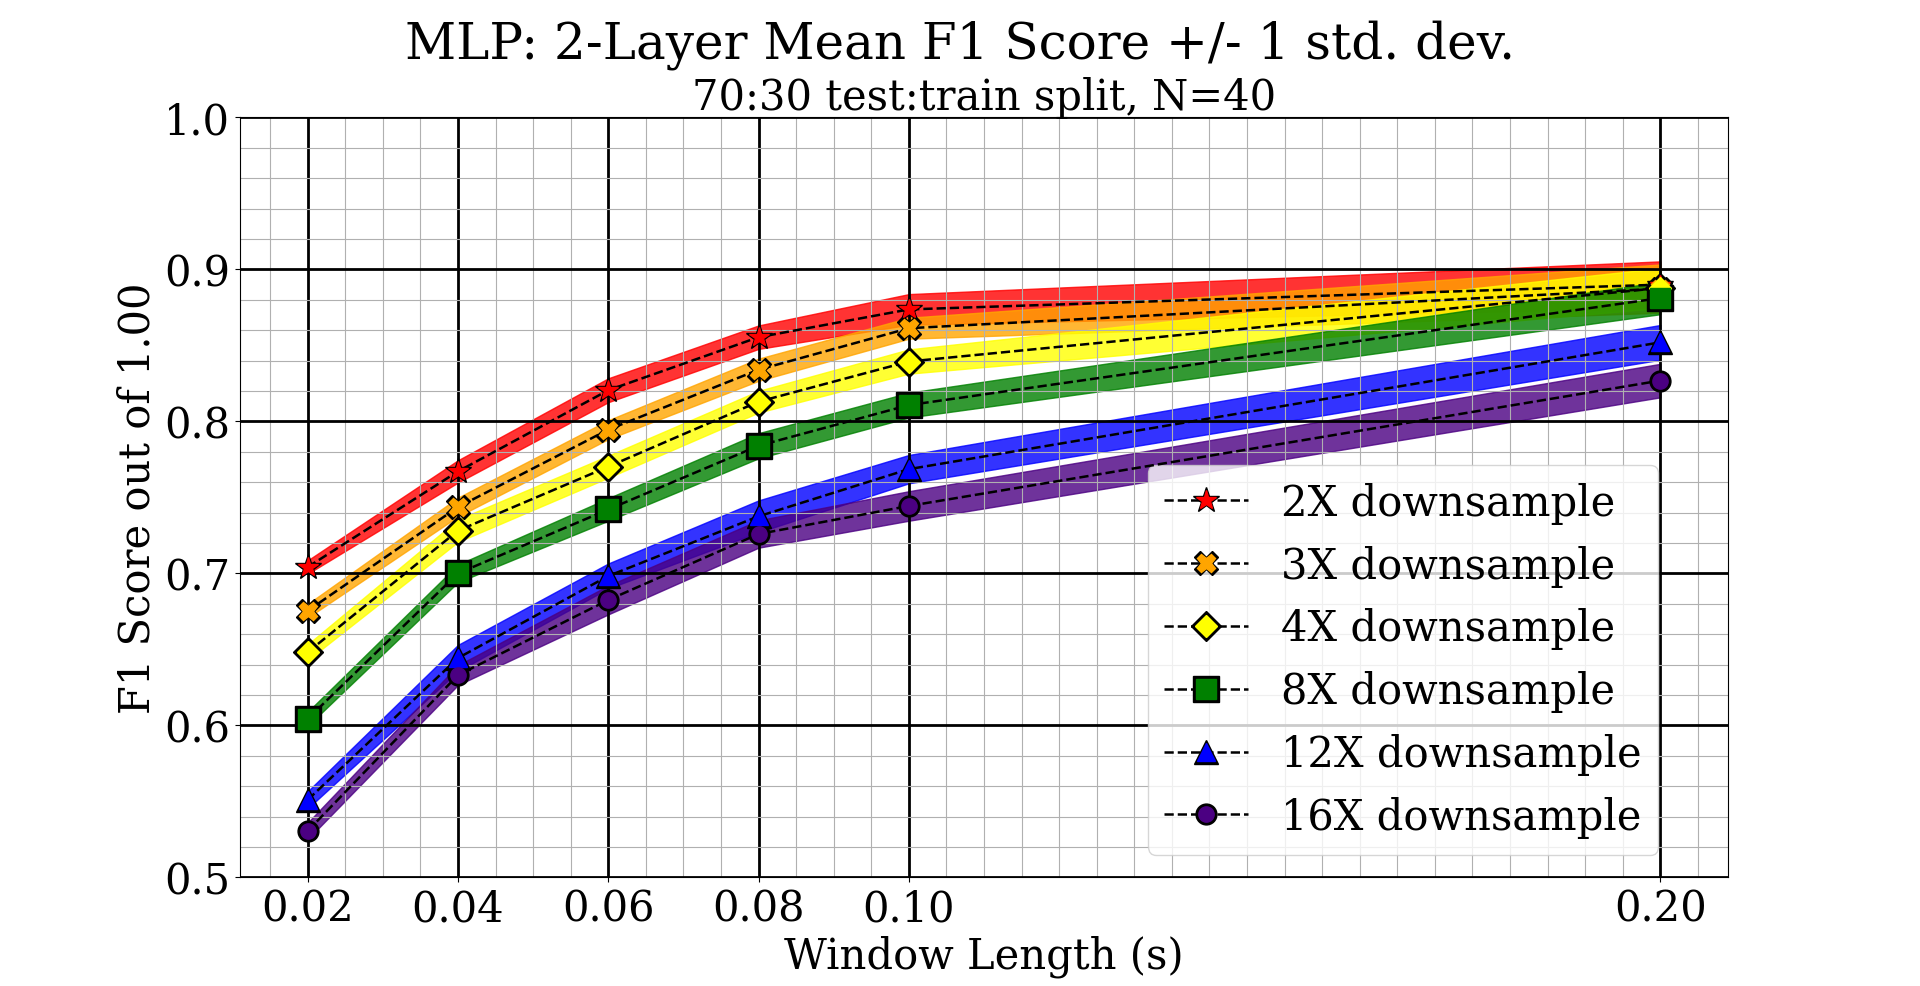
\includegraphics[width=5.5in]{p2_media/figures/raw/MLP_F1_scores.png}
\caption{
The mean F1 score and standard deviation for the tested multi-layer perceptron methods.
This method has the power to classify data very accurately for samples similar to its training data.
Different network sizes are tested to achieve maximum performance.
This method scores similarly to the support-vector machine, but uses more resources.
Both longer window lengths and higher sampling rates, or less downsampling, increased performance.
Increasing window length gave better performance for the number of variables introduced
compared to increasing sampling rates.
Using a window length of 0.2 seconds gave the best performance of for all downsampling levels,
and the score tapered to about 0.90.
}
\label{fig:perf_MLP}
\end{figure}


\subsection{Discussion}

It is well known that changes in tool wear produce changes in vibrational response
across many domains. This fact is also true in the case of underground mining. 
Human operators use sound cues as one of the means of assessing tool wear during operation.
The operators have many duties, and this skill can be difficult to train, 
since the process is subjective. By providing operators a means to perform some of these
duties from a safer position, their exposure to risks at the mining interface can be reduced
\cite{Bartels2009}. 
We propose the addition of objective acoustic data collection and analysis to aid in tool wear classification.

When using methods like the ones described in this work, the cutting conditions must be taken into account.
For example, cutting different materials can also produce different modal responses as well as cutting
at different speeds, penetrations, and with different tool geometries. The operators ability to deduce
changes in wear in different materials comes from experience in cutting those materials with tools at 
different wear levels. Likewise, to successfully apply this technique, data would need to be captured
and analyzed for different cutting conditions.

When comparing the methods for implementation in the application, the support-vector machine
would be an efficient classifier to use, as it scores as well as the multi-layer perceptron classifier,
but has reduced computational complexity. Our results also indicate that longer sample times, which 
give increased resolution for the sampled frequencies, provides better classification performance than
using an increased sampling rate for a shorter duration considering the number of variables introduced.
%This effect continued even with longer sample duration and greater downsampling rates than presented here.

With a window of 0.2 seconds, the tested sampling rates had similar performance.
At this sample length, the input dimension is large, especially when little downsampling is used.
Use of larger samples was computationally infeasible for our equipment and 
also would also have reduced the number of samples available in our data set.
The good performance of signals with long duration and downsampling
implies that lower frequencies are of particular interest for tool wear classification in rock cutting.
The code and data used for this work are available at:
\url{https://github.com/Fworg64/concrete_tool_wear}.

After classification, human operators could be alerted to the anomalous conditions 
to allow them to make a decision to either stop the operation
for further diagnostics or continue cutting if they know from experience 
what could be causing a false positive or how long to extend the current operation.
Also, this technology that can monitor tool wear in an objective manner
would provide a mechanism to monitor the performance of human operators. 
This can help operators and other stakeholders identify areas where they can improve.
It can also be used to assist in training and help to identify risky operation.
Either way, the feedback could be collected from a greater distance, 
reducing the operators exposure to dust and other hazards.

To implement this technology, only a simple and low-cost microphone would need to be placed near
the cutting interface to detect the mode shifts associated with changing tool wear. These devices
are low power, low cost, and very portable, making them well suited for the mining environment.
However, since the signal is only collected from one or maybe several points, it is unlikely that
this technology could predict which tools are worn on the drum head. Also, interference from nearby
operations which are producing noise could also affect the accuracy of this method were it to be
deployed to an active mine. Ultimately, this technology could assist operators in performing their
role from a greater distance and provide a level of objective feedback that is not currently present.


\subsection{Conclusion}\label{sec13}

In this paper, we showed a method for classifying the different acoustic signals
generated by conical picks of different wear levels cutting into a controlled concrete sample. 
The changes in tool mass and geometry lead to excitation of different modes,
which can be detected and classified by the tested methods after 
appropriate preprocessing. Of the tested methods,
the support-vector machine using long duration samples that are downsampled to an appropriate dimension, 
like 200 milliseconds and 4 times downsampling,
performs well and is computationally efficient.

Acoustic emissions are currently processed by human operators with many duties. 
By automatically classifying the acoustic emissions, operators
can be enabled to perform their role from a greater distance.
This way they can avoid hearing damage, harmful dust, and machine proximity
while being able to focus on their many other duties.
With sufficient data collection, 
this classification can be performed with a microphone and an embedded processor.


%\backmatter

\subsection{Acknowledgments}

Special thanks to AliseH and Tivali24 for contributions to the python code for running the experiments
and displaying the data. Special thanks to Syd Slouka for helping run the experiments 
and to Carson Malpass for helping design mounts for acoustic sensors. 

\subsection*{Declarations}

\subsubsection*{Funding}
This work was funded by NIOSH Contract
75D30119C05413, “IMPROVING HEALTH AND SAFETY OF
MINING OPERATIONS THROUGH DEVELOPMENT OF THE
SMART BIT CONCEPT FOR AUTOMATION OF MECHANICAL
ROCK EXCAVATION UNITS AND DUST MITIGATION.”

\subsubsection*{Conflict of interest}
The authors declare that there is no conflict of interest.

\subsubsection*{Availability of data and materials}
The data used for this research is available publicly at: \\
\url{https://github.com/Fworg64/concrete_tool_wear}

\subsubsection*{Code availability }
The code used for this research is available publicly at: \\
\url{https://github.com/Fworg64/concrete_tool_wear}

%%===========================================================================================%%
%% If you are submitting to one of the Nature Portfolio journals, using the eJP submission   %%
%% system, please include the references within the manuscript file itself. You may do this  %%
%% by copying the reference list from your .bbl file, paste it into the main manuscript .tex %%
%% file, and delete the associated \verb+\bibliography+ commands.                            %%
%%===========================================================================================%%

%\bibliography{sn-bibliography}% common bib file
